\PassOptionsToPackage{ukrainian,english}{babel}
\documentclass[twocolumn]{el-author}

%\usepackage[...]{...}      This has been commented out as we are not using any additional packages here.  On the whole, they should be unnecessary.
\usepackage{mathtext}
\usepackage[T1,T2A]{fontenc}
\usepackage[english,ukrainian]{babel}
\usepackage{hyperref}
\usepackage{graphicx} %package to manage images
\usepackage[a4paper, total={7in, 9.5in}]{geometry}
\usepackage{makecell}
\usepackage{tasks}
\graphicspath{ {images/} }
\newcommand{\hH}{\hat{H}}
\newcommand{\D}{^\dagger}
\newcommand{\ua}{\uparrow}
\newcommand{\nc}{\newcommand}
\renewcommand\theadfont{\normalsize\scshape}
\nc{\da}{\downarrow} \nc{\hc}{\hat{c}} \nc{\hS}{\hat{S}}
\nc{\bra}{\langle} \nc{\ket}{\rangle} \nc{\eq}{equation (\ref}
\nc{\h}{\hat} \nc{\hT}{\h{T}}\nc{\be}{\begin{eqnarray}}
\nc{\ee}{\end{eqnarray}}\nc{\rd}{\textrm{d}}\nc{\e}{eqnarray}\nc{\hR}{\hat{R}}\nc{\Tr}{\mathrm{Tr}}
\nc{\tS}{\tilde{S}}\nc{\tr}{\mathrm{tr}}\nc{\8}{\infty}\nc{\lgs}{\bra\ua,\phi|}\nc{\rgs}{|\ua,\phi\ket}
\nc{\hU}{\hat{U}}\nc{\lfs}{\bra\phi|}\nc{\rfs}{|\phi\ket}\nc{\hZ}{\hat{Z}}\nc{\hd}{\hat{d}}\nc{\mD}{\mathcal{D}}
\nc{\bd}{\bar{d}}\nc{\bc}{\bar{c}}\nc{\mc}{\mathcal}\nc{\ea}{eqnarray}\nc{\mG}{\mathcal{G}}\nc{\bce}{\begin{center}}
\nc{\ece}{\end{center}}
\date{20 Грудня 2018}

\begin{document}

\title{Дослідження спектрального складу люмінесценції кристалофосфору}

\author{Сергій Поліщук}

\maketitle

\section{Мета роботи}

 опанування методикою люмінесцентних досліджень.

\section{Прилади і матеріали}

монохроматор УМ-2, ртутна лампа, блок живлення
ртутної лампи, фотопомножувач, блок живлення
фотопомножувача, мікроамперметр .

\section{Завдання}

\begin{enumerate}
	\item при домашній підготовці:
	\begin{itemize}
		\item  користуючись рекомендованою літературою, вивчити
основні закономірності люмінесценції ;
		\item  з методичної розробки до роботи описати у робочому зошиті
установку, метод приготування люмінофору, оптичну схему
монохроматора;
		\item  вивчити будову і принцип дії фотопомножувача.
	\end{itemize}
	\item при виконанні роботи:
	\begin{itemize}
		\item  скласти електричну схему і показати її викладачеві для
перевірки;
		\item  приготувати кристалофосфор;
		\item  дослідити залежність інтенсивності люмінесценції
кристалофосфору від довжини хвилі;
		\item  оформити звіт і подати його викладачеві.
	\end{itemize}
	
\end{enumerate}

\section{Правила техніки безпеки}

\begin{itemize}
	\item  підчас приготування ельфів бережіться оліків ;
	\item  бережіть очі від випромінювання ртутної лампи;
	\item  будьте уважні при використанні блоків живлення
фотопомножувача (напруга близько 1 кВ) та ртутної лампи
(напруга 220 В).
\end{itemize}

\section{Теоретичні відомості та опис установки}

Люмінесценція - випромінювання, що являє собою надлишок над
тепловим випромінюванням тіла при даній температурі і яке має тривалість,
що значно перевищує період світлових коливань.

Ознака протяжності світіння однозначно відрізняє люмінесценцію не
лише від рівноважного теплового випромінювання, а й від інших -
нерівноважних процесів. Ця ознака дає можливість надійного
експериментального розмежування люмінесценції від інших  видів
випромінювання. Незважаючи на достатньо широкий часовий інтервал
тривалості люмінесценції (для різних тіл від $10^{-9}$с до $10^{6}$с), вона все ж
протікає значно довше, ніж період власного коливання молекули, що
світиться ($10^{-14} - 10^{-15}$с).

Умовно розрізняють два типи глюмінесценції: флуоресценцію і
фосфоресценцію. Тривалість післясвічення (часу повного припинення
свічення після  принунинамя збудження) у першому випадку $10^{-8}$с - $10^{-5}$с, 
у другому від $10^{-4}$с до декількох діб.

Для виникнення люмінесценції речовині попередньо потрібно надати
енергію - збудити свічення. Існують різні методи такого збудження:
ультрафіолетовим і видимим світлом (фотолюмінесценція), за рахунок
протікання хімічних реакцій (хемілюмінесценція), гама-випромінюванням
(радіолюмінесценція), рентгенівським промінням (рентгенолюмінесценція), 
нагріванням (термолюмінесценція), ударом (триболюмінесценція),
бомбардуванням електронами (катодолюмінесценція), електричним розрядом
(електролюмінесценція) та ін. У даній роботі збудження люмінофорів
здійснюється ультрафіолетовим світлом  (фотолюмінесценція), яке
випромінює ртутна лампа.

Хоча до цього часу все ще немає повної теоретичної ясності в
трактуванні явищ люмінесценції конденсованих систем (твердих тіл і рідин),
та все ж зрозуміло, що світло, яке здатне викликати люмінесценцію деякої
речовини, має поглинатись цією речовиною. Довжина хвилі збуджуюючого
світла повинна знаходитись близько середини смуги абсорбції. Так як
остання для рідин і твердих тіл достатньо широка, то в межах смуги
абсорбції можна значно варіювати довжину хвилі збуджуючого світла. При
цьому, як показали дослідження, спектральний склад люмінегюннй не
змінюється.

Колір виникаючого свічення є характерною ознакою люмінесценції.
Він відрізняється від кольору збуджуючого світла, за рахунок чого
полегшується спостереження люмінесценції. Джорджом Стоксом у 1852 році
встановлено правило, згідно якого світло люмінесценції характеризується
більшою довжиною хвилі, ніж поглинуте тілом світло, яке викликає
люмінесценцію. На правилі Стокса базується метод поліпшення умов
спостереження люмінесценції, суть якого полягає в тому, що збудження
здійснюється з невидимим ультрафіолетовим світлом, люмінофор же
випромінює видиме світло.

Багаточисельні досліди показали, ї що чисті речовини не
люмінесціюють. Для одержання люмінофорів необхідно в речовину ввести
певні домішки. Із збільшенням концентрації домішок інтенсивність свічення
спочатку зростає, а потім починає падати, наступає так зване концентраційне
гасіння. У зв'язку з цим, при приготуванні люмінофора необхідно строго
дотримуватись встановленої рецептури.

Склад люмінесцентного випромінювання залежить як від роду
домішок, так і від основної речовини. На цій особливості базується
люмінесцентний аналіз - визначення складу речовини за спектром його
випромінювання. Тверді і рідкі тіла дають смугасті спектри люмінесценції.
Для їх одержання вимірюють залежність інтенсивності люмінесценції від
довжини хвилі. Метою цієї роботи і є знаходження такої залежності.

Не вся поглинута речовиною енергія випромінюється потім у вигляді
енергії люмінесценції. Енергетичним виходом люмінесценції прийнято
називати відношення енергії, що випромінюється, до енергії, що
поглинається  люмінесціюючою речовиною. Ця величина для даного
люмінофору, при інших рівних умовах, залежить від температури. При
досягненні певного значення температури енергетичний вихід починає
зменшуватись, має місце температурне гасіння.

Для значного числа люмінофорів люмінесценція спостерігається тільки
при низьких температурах. У цій роботі досліджуються речовини, що
люмінесціюють і при кімнатній температурі. Їх готують за наступним
рецептом:
10 грам цукру розчинити у 10 грамах води. До розчину добавити 2 мг
фарбника (флуоресцеїну) і добре перемішати розчин. Потім воду необхідно
випарувати і довести температуру суміші слабим рівномірним нагріванням
до 145$^{o}$С. При досягненні вказаної температури, цукровий сироп виливають
на металеву плиту, де він швидко затвердіває в льодяник. Температуру
необхідно витримувати точно, оскільки при більш високій температурі цукор
зазвичай розкладається і буріє. При менших температурах замість льодяника
отримується тягуча маса. В обох випадках інтенсивність люмінесценції різко
знижується. Швидке охолодження сприяє виникненню свічення, тому сироп і
виливають на масивну металеву плиту. Виготовлений таким чином
томінофор може існувати декілька діб, по закінченню цього терміну цукор
кристалізується і люмінесценція зникає. Кристалізація прискорюється, якщо
під час виливання в сироп потрапляють кристалики цукру, який не
розчинився, або пилу. Тому необхідно прийняти міри, що запобігають такому
попаданню.

Схема установки, яка використовується для дослідження
спектрального складу люмінесцентного випромінювання, зображена на
рис.\ref{img:1}. Зразок люмінофору 1, який розташовується на тримачі 2,
збуджується випромінюванням ртутної лампи СВД-І20А 5, яка живиться
змінним струмом від блоку 6. Значення струму не повинно перевищувати 1,2А. 
Його регулювання здійснюється трансформатором блоку живлення.
Ртутна лампа, що являє собою газорозрядну трубку, дає лінійчастий спектр
випромінювання парів ртуті. За допомогою світлофільтра УФС-6 4 з цього
спектру виділяється лінія 365 нм. Ультрафіолетове світло кварцевою лінзою
3 фокусується на зразок і збуджує його свічення. Люмінесцентне
пипромінювання фокусується  конденсором 7 на вхідну щілину
монохроматора УМ-2 8. Прилад УМ-2 являє собою спектральний
монохроматор, призначений для різних дослідних робіт і вирішення ряду
аналітичних задач. Область його спектральної чутливості поширюється від
380 нм до 1000 нм. Оптична схема монохроматора зображена на рис.\ref{img:2}.
Люмінесціююче світло через захисне скло 1 та вхідну щілину 2 потрапляє на
об'єктив коліматора 3 і паралельним пучком проходить через диспергуючу
призму 4. Під кутом 90 градусів до падаючого пучка світла розміщується
вихідна труба монохроматора, яка складається із об'єктива 5, щілини б і
захисного скла 7.

Повертаючи за допомогою вимірного барабана призмовий столик на
різні кути відносно падаючого пучка світла, одержуємо у вихідній щілині
світло різної довжини хвилі, яке проходить через призму в мінімумі
відхилення. Після проходження монохроматора, дисперговане
люмінесцентне випромінювання падає на фотокатод фотоелектричного
помножувача ФЕУ-84 9 (рис.\ref{img:1}). У фотопомножувачі світловий сигнал
перетворюється в електричний. Чим більша інтенсивність падаючого на
фотокатод світлового потоку, тим більший струм фіксує мікроамперметр 11,
тому покази  мікроамперметра будуть пропорційні інтенсивності
люмінесценції.

Фотопомножувач живиться постійним струмом високої напруги від
блоку 10. У зв'язку з цим при виконанні роботи слід строго виконувати
правила техніки безпеки.


%\begin{equation} \label{eq:Einstein}
%hv = A+\frac{m_{e}V_{max}^{2}}{2}
%\end{equation}






\section{Послідовність виконання роботи}

\begin{enumerate}
	\item Приготувати люмінофор.
	\item Виготовити з люмінофору зразок розміром 5х5х3 мм і розмістити
його на препаратотримачі під кутом 45$^{o}$ до вісі монохроматора і
до вісі ртутної лампи.
	\item Рукоятку на трансформаторі ртутної лампи поставити в
положення "0", ввімкнути трансформатор в мережу і,
збільшуючи напругу на трубці ртутної лампи, досягти її
запалювання. Рукояткою трансформатора встановити струм через
лампу 1,2 А. При цьому слід мати на увазі, що по мірі
прогрівання лампи струм, який протікає через неї, зменшується і
лампа може згаснути. У зв'язку з цим, струм, що протікає через
лампу, слід регулювати до повного її прогрівання.
	\item Повністю закрити вхідну щілину.
	\item За допомогою вимірювального барабану, на основі
градуювальної таблиці \ref{tab:1}, встановити довжину хвилі, на яку
припадає максимум в спектрі випромінювання (для
виготовленого  люмінофору вона дорівнює 520 нм, для
стандартного 540 нм).
	\item Ввімкнути в мережу блок живлення фотопомножувача і подати
високу напругу на фотопомножувач. Вона повинна становити
900 В.
	\item Ввімкнути в мережу мікроамперметр.
	\item Повільним розкриттям вхідної щілини встановити світловий
"зайчик" мікроамперметра на поділку 90.
	\item Вимірювальний барабан встановити на позначку, що відповідає
довжині хвилі 380 нм і зняти покази мікроамперметра.
Збільшуючи довжину хвилі, проводити вимірювання через кожні
10 нм до 700 нм.

УВАГА! Для запобігання пошкодження фотопомножувача категорично
забороняється:
	\begin{enumerate}
		\item регулювати: вихідну щілину монохроматора, діафрагму ртутної
лампи, напругу на фотопомножувачі;
		\item переключати діапазони виміру мікроамперметра;
		\item проводити зміну люмінофору при ввімкнутій високій напрузі на
фотопомножувачі.
	\end{enumerate}
	\item Вимкнути високу напругу на фотопомножувачі. Замінити
виготовлений зразок на стандартний і повторити вимірювання
відповідно пунктів 4, 5, 6, 8 і 9.
	\item По закінченню роботи вимкнути із мережі блоки живлення
фотопомножувача, ртутної лампи, мікроамперметра.
	\item Знайти середнє значення струму для кожної довжини хвилі і
побудувати графіки залежності інтенсивності люмінесценції від
довжини хвилі для обох зразків.
\end{enumerate}

\begin{table}[ht]
{\begin{tabular}{|c|c|c|c|}\hline
\thead{нм} & 
\thead{град} & 
\thead{нм} & 
\thead{град} \\\hline
380 & 290 & 550 & 2200 \\\hline
390 & 445 & 560 & 2255 \\\hline
400 & 590 & 560 & 2305 \\\hline
410 & 745 & 580 & 2360 \\\hline
420 & 885 & 590 & 2420 \\\hline
430 & 1030 & 600 & 2470 \\\hline
440 & 1120 & 610 & 2510 \\\hline
450 & 1295 & 620 & 2555 \\\hline
460 & 1410 & 630 & 2590 \\\hline
470 & 1520 & 640 & 2630 \\\hline
480 & 1625 & 650 & 2665 \\\hline
490 & 1720 & 660 & 2705 \\\hline
500 & 1810 & 670 & 2735 \\\hline
510 & 1900 & 680 & 2765 \\\hline
520 & 1975 & 690 & 2790 \\\hline
530 & 2055 & 700 & 2820 \\\hline
540 & 2125 & 710 & 2840 \\\hline
\end{tabular}}{}
\end{table}



\begin{thebibliography}{}

\bibitem{1}
Кучерук І.М., Горбачук І.Т. Загальний курс фізики: Т.3.: Оптика.
Квантова фізика. - К.: Техніка, 2006. -- 518с., ст. 327 - 330.

\bibitem{2}
Кучерук І.М, Дущенко В.П. Загальна фізика. Оптика. Квантова
фізика. - К.: Вища школа, 1991. -- 463с., ст. 340 - 342.

\bibitem{3}
Хмелюк К.Д., Цициліано Д.Д. Фізика атома і твердого тіла. - К.:
Вища школа, 1974. - 231с., ст.201 - 207.

\bibitem{4}
Методична розробка до роботи.

\end{thebibliography}

\section{Завдання для самоконтролю}

\begin{enumerate}
	\item Дайте означення люмінесценції.
	\item Перелічіть методи збудження люмінесценції.
	\item Сформулюйте правило Стокса.
	\item Сформулюйте закон Вавилова.
	\item Де застосовується люмінесцентний аналіз?
	\item Як змінюється інтенсивність люмінесценції з температурою?
	\item При яких умовах відбувається концентраційне гасіння?
	\item Зобразіть зонну схему кристалофосфору?
	\item Чому одержані спектри люміненсценсії смугасті?
	\item Яка будова фотопомножувача?
\end{enumerate}

\clearpage
\begin{figure}[h]
\centering{\includegraphics[width=80mm]{img_1}}
\caption{\source{}}
\label{img:1}
\end{figure}

\begin{figure}[h]
\centering{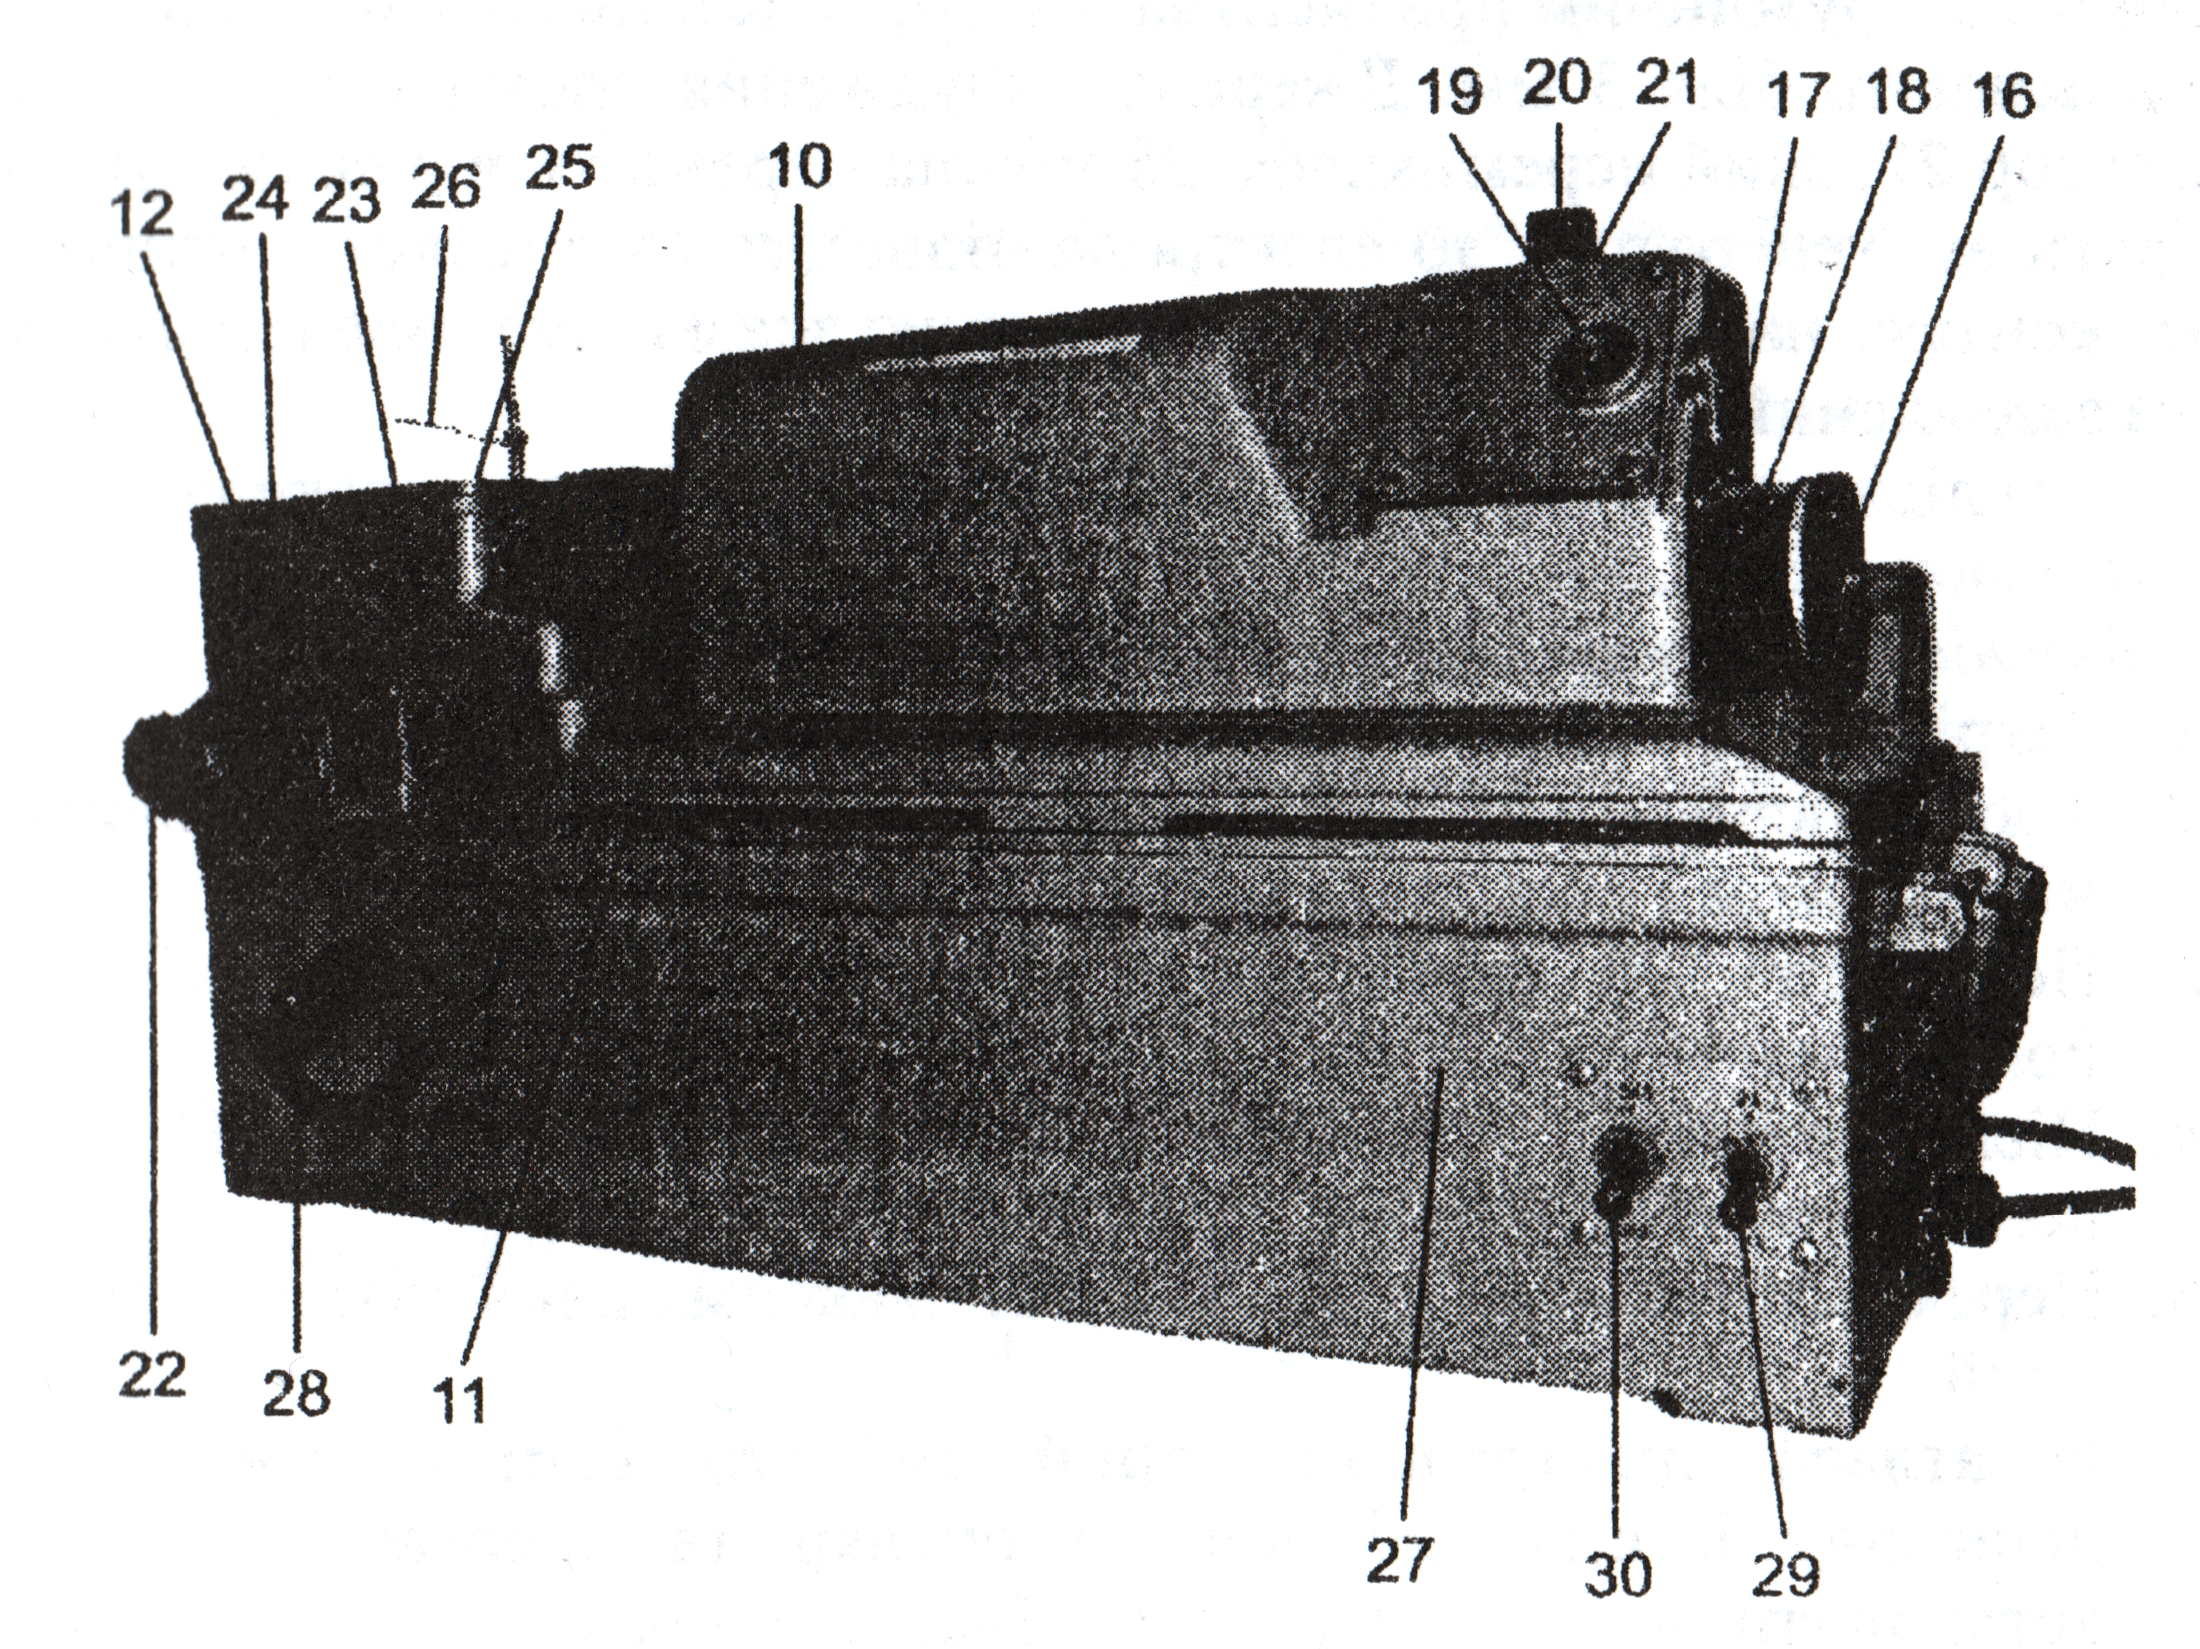
\includegraphics[width=80mm]{img_2}}
\caption{\source{}}
\label{img:2}
\end{figure}

\newpage
\begin{enumerate}
	\item люмінофор;
	\item препаратотримач;
	\item фокусуюча лінза;
	\item світлофільтр УФС-6;
	\item ртутна лампа СВД-120 А;
	\item блок живлення лампи;
	\item конденсор;
	\item монохроматор УМ-2;
	\item фотопомножувач;
	\item блок живлення фотопомножувача;
	\item мікроамперметр;
\end{enumerate}

\bigskip
\bigskip
\bigskip
\bigskip
\bigskip
\bigskip
\bigskip

\begin{enumerate}
	\item захисне скло вхідної щілини;
	\item вхідна щілина;
	\item об'єктив коліматора;
	\item диспергуюча призма;
	\item об'єктив зорової труби;
	\item вихідна щілина;
	\item захисне скло вихідної щілини.
\end{enumerate}


\clearpage
\section{Тестові завдання для вхідного контролю}

\begin{enumerate}
	\item Під кристалофосфорами розуміють:
	\begin{enumerate}
		\item будь-які тверді тіла;
		\item будь-які кристалічні речовини;
		\item неорганічні кристалічні речовини;
		\item органічні кристалічні речовини.
	\end{enumerate}
	\item Ліомінесценцію можна викликати:
	\begin{enumerate}
		\item ударом;
		\item охолодженням;
		\item освітленням;
		\item хімічною реакцією.
	\end{enumerate}
	\item Яке з цих тверджень хибне? Фосфоресценція притаманна:
	\begin{enumerate}
		\item виключно газам;
		\item лише рідинам;
		\item переважно твердим тілам;
		\item усім агрегатним станам.
	\end{enumerate}
	\item При флуоресценції і фосфоресценції тривалість післясвічення:
	\begin{enumerate}
		\item приблизно однакова;
		\item може бути як більшою, так і меншою;
		\item для флуоресценції менша;
		\item для фосфоросценції менша.
	\end{enumerate}
	\item Із правила Стокса слідує наступне співвідношення між довжиною хвилі
	$\lambda_{люм}$, що відповідає максимуму у смузі люмінесценції, і довжиною хвилі
	$\lambda_{зб}$, що відповідає максимуму у смузі збудження:
	\begin{enumerate}
		\item $\lambda_{люм} = \lambda_{зб}$;
		\item $\lambda_{люм} > \lambda_{зб}$;
		\item $\lambda_{люм} < \lambda_{зб}$;
		\item у залежності від умов спостереження може бути як 
		$\lambda_{люм} < \lambda_{зб}$, так і $\lambda_{люм} > \lambda_{зб}$
	\end{enumerate}
	\item Причиною антистоксового свічення є:
	\begin{enumerate}
		\item  порушення закону збереження енергії у люмінесцентних явищах;
		\item двохфотонне збудження (енергії двох налітаючих на люмінофор фотонів
складаються);
		\item додавання до енергії  збуджуючого фотона теплової енергії
люмінесціюючої речовини;
		\item невідомі дотепер явища.
	\end{enumerate}
	\item Після припинення збудження кристалофосфора інтенсивність його
свічення згасає з часом:
	\begin{enumerate}
		\item за експоненціальним законом;
		\item за гіперболічним законом;
		\item лінійно;
		\item за параболічним законом.
	\end{enumerate}
	\item  Чи впливають на люмінесценцію кристалів домішки?
	\begin{enumerate}
		\item суттєво не впливають;
		\item наявність домішок у будь-якій концентрації гасить світіння;
		\item уведення домішок завжди підсилює люмінесценцію;
		\item при малих концентраціях домішок яскравість люмінесценції зростає, а
при значних -- зменшується аж до повного гасіння.
	\end{enumerate}
	\item Якщо кристалофосфор охолоджувати, то інтенсивність його
люмінесценції:
	\begin{enumerate}
		\item суттєво не змінюватиметься;
		\item буде швидко зменшуватися;
		\item спочатку буде зменшуватися, а при досягненні певної температури
почне збільшуватися;
		\item буде зростати.
	\end{enumerate}
	\item У даній роботі фотопомножувач живиться напругою, порядок якої
	\begin{enumerate}
		\item 10 В;
		\item 100 В;
		\item 1000 В;
		\item 10000 В.
	\end{enumerate}
\end{enumerate}

\section{Тестові завдання для підсумкового контролю}

\begin{enumerate}
	\item При люмінесценції:
	\begin{enumerate}
		\item $t = T$;
		\item $t > T$;
		\item $t < T$;
		\item $t \approx T$.
	\end{enumerate}
	де $t$ - тривалість люмінесценсії, $T$ - період власних коливань молекули, що
світиться.
	\item Флуоресценція спостерігається у:
	\begin{enumerate}
		\item газах;
		\item лише в рідинах;
		\item виключно у твердих тілах;
		\item переважно у газах і рідинах.
	\end{enumerate}
	\item Світло, яке здатне викликати люмінесценцію деякої речовини, повинно:
	\begin{enumerate}
		\item поглинатися цією речовиною;
		\item проходи через цю речовину;
		\item розсіюватися цією речовиною;
		\item відбиватися від цієї речовини.
	\end{enumerate}
	\item Який з нижче наведених законів збереження енергії відповідає правилу
Стокса?
	\begin{enumerate}
		\item $hv = A + \frac{mV^{2}}{2}$;
		\item $\frac{mv^{2}}{2} = Q + hv$;
		\item $hv + m_{o}c^{2} = hv_{1} + mc^{2}$;
		\item $hv = A + hv_{1}$.
	\end{enumerate}
	\item Закон Стокса-Ломмеля формулюється так:
	\begin{enumerate}
		\item спектр люмінесценції і його максимум зміщені в бік довших хвиль
порівняно зі спектром поглинання і його максимумом;
		\item спектр люмінесценції і його максимум зміщенні в бік коротших хвиль
порівняно зі спектром поглинання і його максимумом;
		\item спектр люмінесценції і його максимум співпадають зі спектром
поглинання і його максимумом;
		\item спектр люмінесценції і його максимум не залежать від спектру
поглинання і його максимума.
	\end{enumerate}
	\item Чи змінюються інтенсивності | стоксового і  антистоксового
випромінювання зі зміною температури кристалофосфора?
	\begin{enumerate}
		\item температурна залежність відсутня;
		\item зі зменшенням температури зростає лише стоксове випромінювання,
		інтенсивність антистоксового не змінюється;
		\item інтенсивність обох випромінювань при збільшенні температури зростає;
		\item з підвищенням температури інтенсивність стоксового випромінювання
зменшується, а антистоксового збільшується.
	\end{enumerate}
	\item Які з нижче перелічених елементарних процесів притаманні
	люмінесценції: 1)~резонансний 2)~спонтанний, 3)~вимушений,
4)~рекомбінаційний?
	\begin{enumerate}
		\item лише останній;
		\item третій і четвертий;
		\item перший, другий і третій;
		\item всі чотири.
	\end{enumerate}
	\item Квантовий вихід люмінесценції:
	\begin{enumerate}
		\item завжди менший одиниці;
		\item завжди рівний одиниці;
		\item може бути більшим одиниці;
		\item може бути меншим одиниці, рівним одиниці і більшим одиниці.
	\end{enumerate}
\end{enumerate}

\end{document}

%\begin{table}[b]
%\processtable{Coefficients and remainders for distribution KK ($k = 0.05$,
%$v = 3$, $c_{1} = 1.5$, $c_{2} = 4.5$)}
%{\begin{tabular}{|l|l|l|}\hline
%$n$ & $a_{n}^{2}$ & $r_{k}(1)$\\\hline
%0 & 3.602576748428 & 1.493719547999\\\hline
%1 & 1.384791111989 & 0.108928436101\\\hline
%2 & 0.108600438794 & 0.000327997399\\\hline
%3 & 0.000275794597 & 0.000052202814\\\hline
%4 & 0.000027616892 & 0.000024585922\\\hline
%5 & 0.000018178621 & 0.000006407300\\\hline
%\end{tabular}}{}
%\end{table}
%
%So, the basic preamble and main body will be:
%\verb"\documentclass[twocolumn]{el-author}"\\
%\verb"\usepackage[...]{packages}"\\
%\verb"\date{12 December 2012}"\\
%\verb"\title{...}"\\
%\verb"\author{...}"\\
%\verb"\abstract{...}"\\
%\verb"\maketitle{...}"\\
%\verb"\begin{document}"\\
%\verb"..."\\
%\verb"\section{...}"\\
%\verb"..."\\
%\verb"\section{..}"\\
%\verb"..."\\
%\verb"\end{document}"